\newpage
\section{Dataset analysis and preprocessing}
\subsection{Dataset description}
The provided dataset contains 10000 points with 10 features named from $x1$ to $x10$ and a label column named $y$.\\
All the feature are floating point values and the dataset is well formed (in the sense that there are no missing values).\\
The label column contains values that are either $-1$ or $+1$.\\
There isn't any duplicated data in the training set.\\
I collect the major statistics from each feature in the dataset: \textit{mean}, \textit{standard deviation}, \textit{min} and \textit{max}.\\

\begin{center}
    \begin{tabular}{| c | c | c | c | c | c |}
    \hline
     & x1 & x2 & x3 & x4 & x5 \\
    \hline
    min & 2.44342055e-03 & -7.52493399e+00 &  9.85724553e+01 & -7.07893888e+00 & -9.99999717e-01  \\
    \hline
    max & 9.38422309e+00 &  8.30237476e+00 &  1.01260768e+02 & -2.92150729e-06 & 9.99999998e-01 \\
    \hline
    mean & 1.59129826e+00 &  5.15879411e-01 &  9.98489361e+01 & -1.50413876e+00 & 7.76447773e-02 \\
    \hline
    std & 1.32111881 & 2.05438485 & 0.71091203 & 1.13354878 & 0.70723419 \\
    \hline
    \end{tabular}
\end{center}

\begin{center}
    \begin{tabular}{| c | c | c | c | c | c |}
    \hline
     & x6 & x7 & x8 & x9 & x10 \\
    \hline
    min  & -6.90697075e+00 & -7.14075517e+00 & -7.15188951e+00 & -5.67739307e+01 & -1.00000000e+00 \\
    \hline
    max &  8.76030588e+00 &  9.28726632e+00 & 6.21145227e+00 & -5.42088897e+01 & 1.00000000e+00 \\
    \hline
    mean &  5.18228648e-02 &  9.75207134e-01 &  6.35194433e-01 & 5.19260973e-02 & -5.54476783e+01 \\
    \hline
    std & 0.70471943 & 2.16212877 & 2.21259701 & 1.76955726 & 0.71004639 \\
    \hline
    \end{tabular}
\end{center}

It's clear from the main features that the different features have different ranges and follow different probability distributions.

\subsection{Feature Scaling}
Because the dataset is already well formed and there are no missing values the first thing I do is scale the features.\\
This step should ensure that the values of the features are in a comparable range.\\
I tried two approaches: normalization and standardisation.\\
\textbf{Standardization} sets each feature to have a mean of 0 and a standard deviation of 1.\\
This is achieved by subtracting the feature mean from each value and dividing by its standard deviation:
$$x' = \frac{x - \mu}{\sigma} $$
(where $\mu$ is the mean and $\sigma$ is the standard deviation).\\
In the case of \textbf{normalization}, the features are rescaled in a fixed range between 0 and 1 in the following way: $$x' = \frac{x - x_{min}}{x_{max} - x_{min}} $$.\\
It's important to note that we should perform both approaches using a sound procedure, more specifically, we should avoid data leakage:
When calculating the minimum and maximum of the feature, we should only consider the training set and scale the test set only according to these values, without deriving any information from it.\\
In the same way, we should calculate the mean and standard deviation for the standardization process.\\
Both of these approaches lead to important improvements and can be demonstrated both from an empirical point of view (see table \ref{tab:scaling}) and from a theoretical perspective (explained in the chapter describing perceptron).
It's also worth noting that I couldn't run the logistic regression without first rescaling the data, due to a float overflow in the exponentiation for the sigmoid function.\\

\begin{center}
    \begin{tabular}{| c | c | c | c |}
    \hline
    & None & Normalization & Standardization  \\
    \hline
    Perceptron & 0.507 & 0.482 & 0.326  \\
    \hline
    Pegasos & 0.294 &  0.2805 & 2807 \\
    \hline
    \end{tabular}\\
    \label{tab:scaling}
    Comparison of test errors between Perceptron and Pegasos with the three different scaling options.\\
\end{center}

Is possible to choose which scaling method use with the cli option \textit{\-\-preprocess} and choose between\textit{none}, \textit{normalize} and \textit{standardize}.\\
I used the standardization methods by default because is the one that perform better in the majority of the cases.\\



\subsection{Outliers removal}
Another approach I considered is removing the outliers from the dataset using the Z-score methods.\\
I calculated the score $ Z = (x - \mu) / \sigma$ for each value where $\mu$ is the mean and $\sigma$ is the variance of the feature.\\
I then removed all the points with a Z-score greater or equals than $3$ in absolute value.\\
I found (and removed) 265 outliers (recall that the dataset has size 10000).\\
I tried training non-kernelized Perceptron and Pegasos over the modified dataset but the results shows that the dataset is already sufficently cleaned: in fact it  
affects the performance of the models in a minimum way with no significative changes, and even in some cases it is (even if only slightly) worsening\\

\begin{center}
    \begin{tabular}{| c | c | c |}
    \hline
    & with outliers & without outliers \\
    \hline
    Perceptron & 0.326 & 0.326 \\
    \hline
    Pegasos & 0.2865 &  0.29  \\
    \hline
    Feature expanded Perceptron &  0.087 & 0.087 \\
    \hline
    Feature expanded Pegasos & 0.0555 & 0.0565  \\
    \hline
    \end{tabular}\\
    Comparison of test errors (using zero one loss) with and without outliers.\\
    Note that when I refere to feature expansion I intend polynomial feature expansion of degree 2.\\
\end{center}

Is possible to enable the outliers removal using the cli flag \textit{\-\-remove-outliers}.\\

\subsection{Feature correlation}
I sorted all the point according to each axis and plot on the other axis all the other features to spot eventual correlation and I observed that the feature \textit{x2} and \textit{x5} have a linear correlation (with a negative coefficent, see Fig. \ref{fig:corr25}) as the feature \textit{5} and \textit{9} (with positive coefficent, see Fig. \ref{fig:corr59}).\\ 

\begin{figure}[h]
    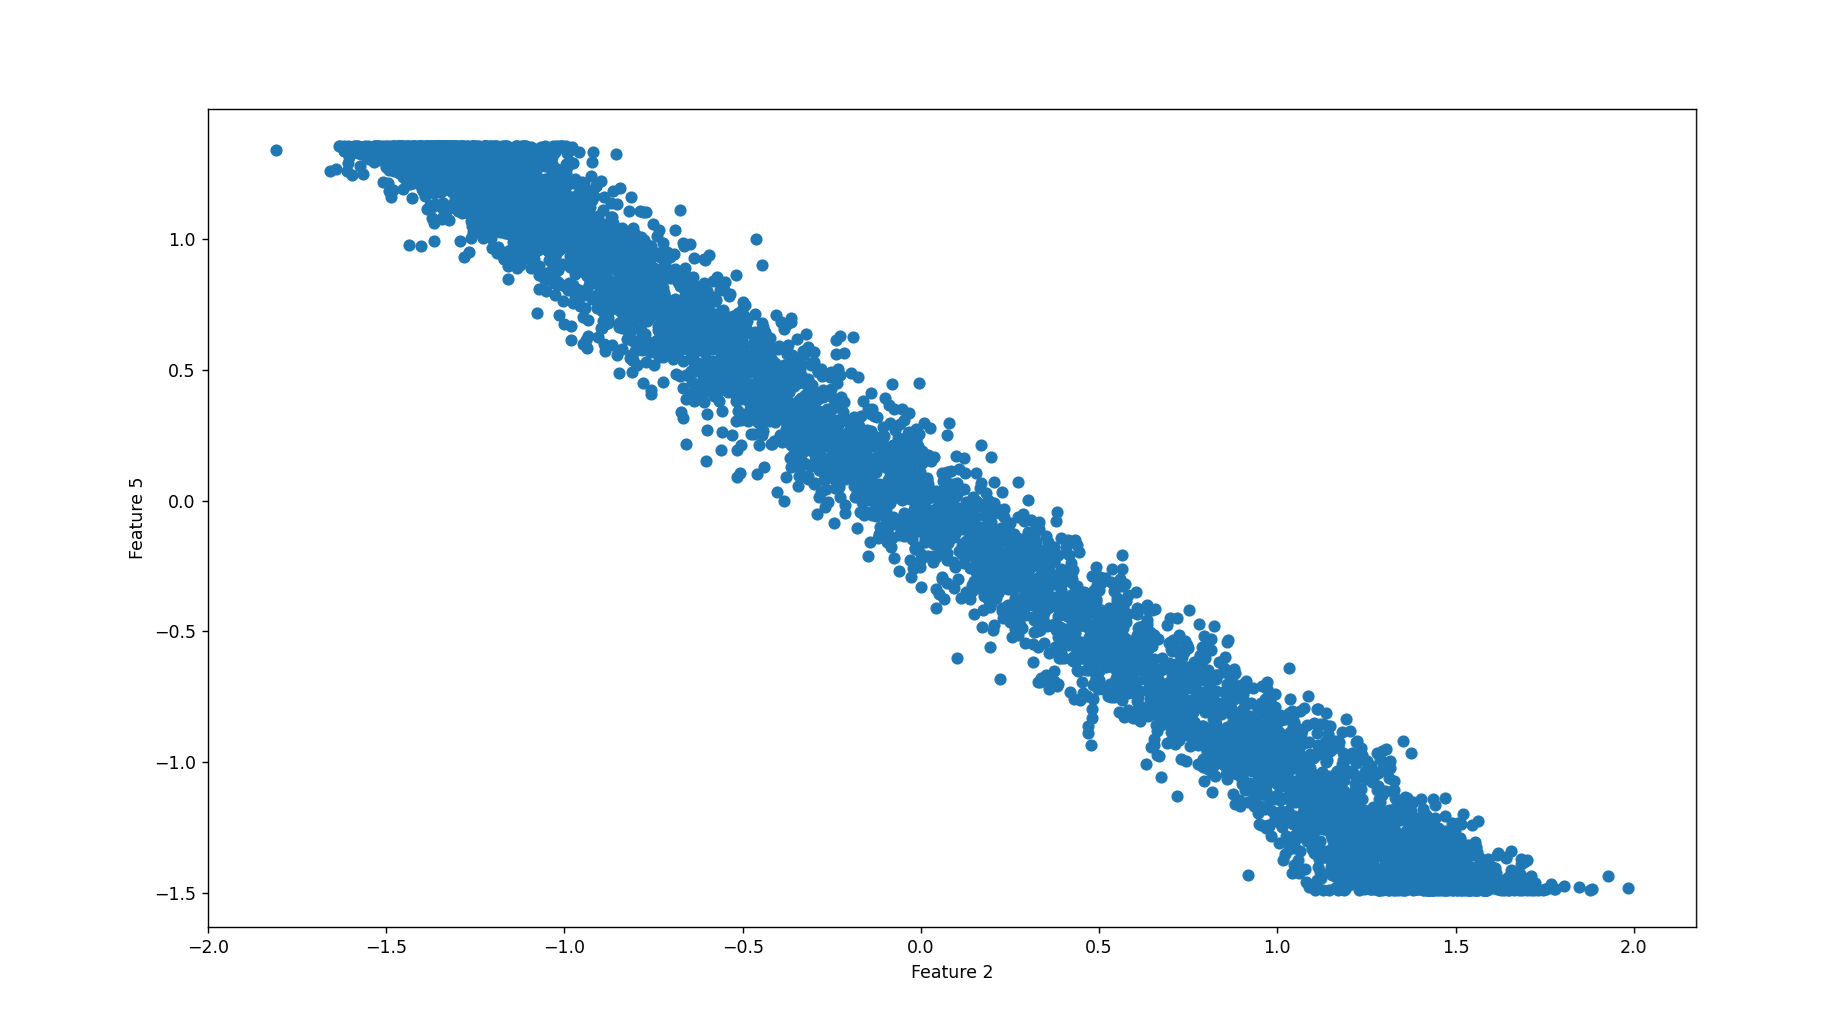
\includegraphics[width=\textwidth]{images/feature_2_5_correlation.png}
    \caption{Here there is a clear linear correlation between feature \textit{x2} and \textit{x5}, but very noisy}
    \label{fig:corr25}
\end{figure}

\begin{figure}[h]
    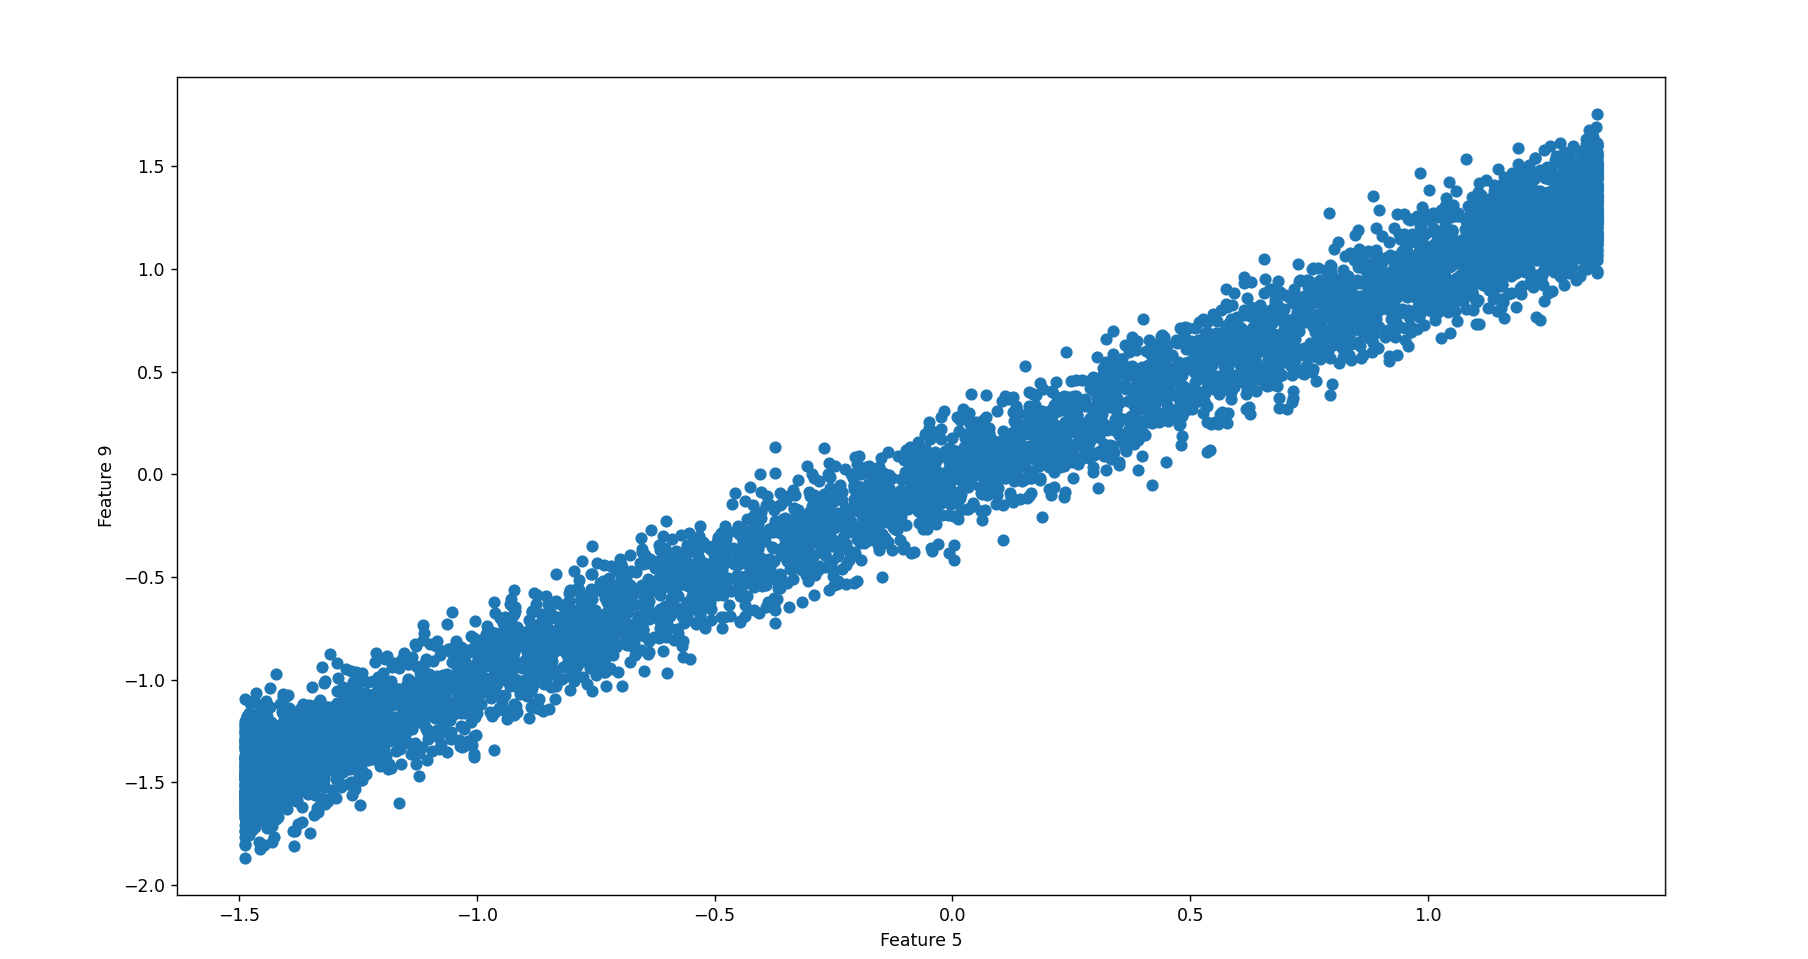
\includegraphics[width=\textwidth]{images/feature_5_9_correlation.png}
    \caption{Another correlation is also present between feature \textit{x5} and \textit{x9} (with a negative coefficent)}
    \label{fig:corr59}
\end{figure}

One possibility in this case during the preprocessing of the data is to remove the correlated features and leave only one of them to avoid redundancy of the data.\\
I don't follow this approach because there is a sensibile noise in the correlation and removing some features can lead to also removing this noise that can encode important information for the model.\\


\subsection{Feature expansion}
To being able to express non-homogeneous linear separators (hyperplane that don't pass through the origin) I add a constant feature of value $1$ to each point in the dataset.\\
Let $\bf(x)$ be any point in the dataset and $\bf(w)$ be the linear separator, if we define $x' = ({\bf x}, 1)$ we can define $w' = ({\bf} w, c)$, in that way: $${w'}^T x' = ({\bf w}^T {\bf x} + c)$$\\
